\subsection{Defini\c{c}\~oes de seguran\c{c}a}
\label{subsection:definicoes_seguranca}
Como \cite{o2003comparing} fala em seu artigo as defini\c{c}\~oes relativas aos sistemas e m\'etodo em seguran\c{c}a s\~ao definidas como forte ou fraca. Isso acontece pois quando usamos termos relativos, segundo o mesmo, somos claros na mensagem que queremos passar a respeito da informa\c{c}\~ao. Por exemplo, quando dizemos que uma porta com uma trava \'e mais segura, mais forte, que uma porta que n\~ao possui trava alguma, relativamos a seguran\c{c}a da trava tornando claro a mensagem que por mais que seja mais segura n\~ao \'e imposs\'ivel de ser quebrada.
\paragraph{}
Por mais que a relativiza\c{c}\~ao muitas vezes seja vista com maus olhos no campo da inform\'atica a garantia de um sistema inviol\'avel \'e quase imposs\'ivel e quando poss\'ivel altamente custoso. 
\paragraph{}
Como podemos ver no livro do \cite{stuttard2011web} h\'a diversas maneiras de se burlar um sistema web por exemplo, mesmo sendo um sistema altamente visado e onde pessoas se preocupam o tempo todo em proteg\^e-lo. Mas um ponto comum de quase todo ataque \'e o qu\^e conhecemos como engenharia social. A entrada sempre acontece por meio de pessoas, ou fragilidade dessas pessoas.
\paragraph{}
\'E muito dif\'icil mensurar seguran\c{c}a em termos absolutos. Uma forma de mensurar \'e atrav\'es da for\c{c}a e da fraqueza de um sistema. Um sistema forte \'e aquele que o custo de atacar \'e muito maior que o ganho o atacando. Ou seja, o trabalho para consegui a informa\c{c}\~ao vai ser t\~ao grande que n\~ao compensar\'a. Um exemplo \'e em \cite{biryukov2010key} a alta complexidade e tempo para se quebrar uma chave AES-256.
\paragraph{}
Paralelamente \`a isso temos a fraqueza de um sistema. Essa \'e o oposto da for\c{c}a. Ou seja, o custo de ataque \'e menor do o ganho obtido com os resultados. E de que custo podemos entender n\~ao s\'o dinheiro como tamb\'em tempo, potencial para puni\c{c}\~ao criminal e etc.
\paragraph{}
Mas focando em aplica\c{c}\~oes que utilizem CDN como distribui\c{c}\~ao podemos elencar os principais pontos de sua seguran\c{c}a conforme analisado por \cite{pomelo2009analysis}.
\paragraph{}
Precisa-se primeiro listar as principais premissas para se garantir que um sistema de distribui\c{c}\~ao de multim\'idia, como o netflix, possa ser considerado fortemente seguro.
\begin{itemize}
\item Apenas os usu\'arios com o devido acesso podem acessar determinados conte\'udos;
\item Os usu\'arios n\~ao podem compartilhar suas informa\c{c}\~oes com outros;
\item Os conte\'udos s\'o podem ser acessados para regi\~oes espec\'ificas. Usu\'arios americanos s\'o podem acessar conte\'udos americanos.
\item O conte\'udo n\~ao pode ser redistribu\'ido e reutilizado sem verificar novamente as credenciais de acesso.	 
\end{itemize}

Quanto a esses itens podem ser tomadas diversas precau\c{c}\~oes. Mas partindo da ideia do esforço m\'inimo com o m\'aximo de ganho, podemos destacar algumas atividades que podem cobrir esses casos de usos e deixar o sistema seguro. Precau\c{c}\~oes essas que s\~ao:
\begin{itemize}
\item Fazer a requisi\c{c}\~ao de autentica\c{c}\~ao de usu\'ario momentos antes de tocar o v\'ideo;
\item Limitar o n\'umero de acessos simult\^aneos ao servi\c{c}o por usu\'ario;
\item Bloquear acessos de IPs de fora do \textit{range} da regi\~ao delimitada;
\item Encriptar o conte\'udo;
\item Promovendo um \'unico par de chaves entre conte\'udo e \textit{device}.
\end{itemize}

Essas s\~ao apenas algumas a\c{c}\~oes que se pode tomar para evitar vazamento de informa\c{c}\~ao desejada em uma CDN voltada para a distribui\c{c}\~ao de conte\'udo.
\paragraph{}
Para garantir que esses pontos sejam de fato cobertos a netflix utiliza de um esquema, explicado em \cite{pomelo2009analysis}, que conta com quatro servidores distintos que possuem objetivos bem especificados.
\begin{itemize}
\item \textit{Individualization server};
\item \textit{Web services};
\item servidor de controle;
\item e servidor de \textit{streaming}.  
\end{itemize}
Os objetivos desses servidores podem ser verificados na figura \ref{figura:servidores_netflix}:
\begin{figure}[H]
\caption{Rede de servidores netflix}
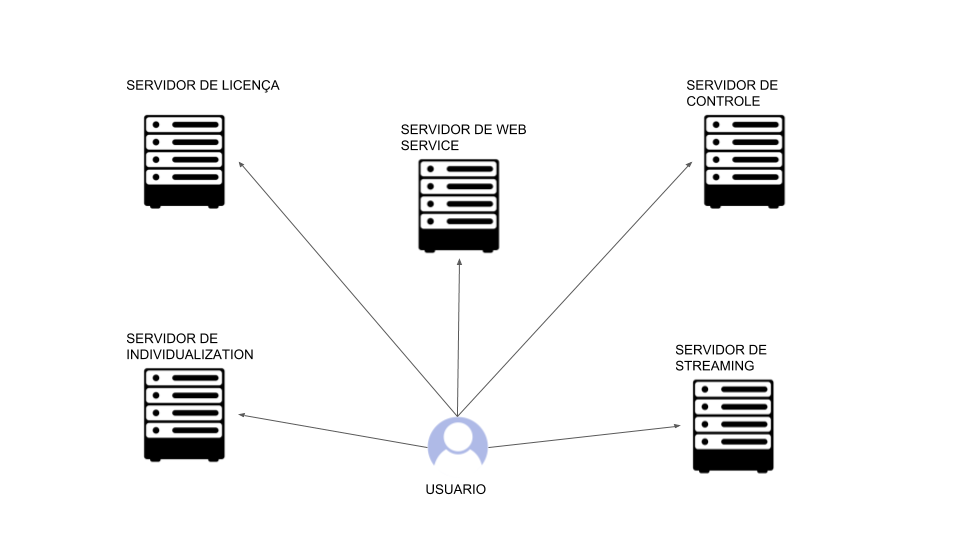
\includegraphics[width=14cm]{Figuras/servidores_netflix.png} 
\label{figura:servidores_netflix}
\end{figure}